\documentclass{beamer}
\usepackage[utf8]{inputenc}

\usetheme{Madrid}
\usecolortheme{default}
\usepackage{amsmath,amssymb,amsfonts,amsthm}
\usepackage{txfonts}
\usepackage{tkz-euclide}
\usepackage{listings}
\usepackage{adjustbox}
\usepackage{array}
\usepackage{tabularx}
\usepackage{gvv}
\usepackage{lmodern}
\usepackage{circuitikz}
\usepackage{tikz}
\usepackage{graphicx}

\setbeamertemplate{page number in head/foot}[totalframenumber]

\usepackage{tcolorbox}
\tcbuselibrary{minted,breakable,xparse,skins}

% Code styling
\lstset{
    language=C,
    basicstyle=\ttfamily\small,
    keywordstyle=\color{blue},
    stringstyle=\color{orange},
    commentstyle=\color{green!60!black},
    numbers=left,
    numberstyle=\tiny\color{gray},
    breaklines=true,
    showstringspaces=false,
}
%------------------------------------------------------------

\title
{4.4.4}
\author 
{AI25BTECH11008\\Chiruvella Harshith Sharan}

\documentclass{beamer}
\usepackage{amsmath, amssymb}
\usepackage{mathtools}

\title{4.4.4}
\author{AI25BTECH11008 - Chiruvella Harshith Sharan}
\date{}

\begin{document}

\frame{\titlepage}

\begin{frame}{Question}
\centering
A line passes through the point with position vector
\[
\vec{A} = 2\hat{i} - \hat{j} + 4\hat{k}
\]
and is in the direction of the vector
\[
\vec{d} = \hat{i} + \hat{j} - 2\hat{k}.
\]
Find the equation of the line?
\end{frame}

\begin{frame}{Theoretical Solution}
\vspace{0.4cm}

The given point and direction vector are:
\begin{equation}
\vec{A} = \myvec{2 \\ -1 \\ 4}
\end{equation}
\begin{equation}
\vec{d} = \myvec{1 \\ 1 \\ -2}
\end{equation}

The vector equation of a line is
\begin{equation}
\vec{r} = \vec{A} + \lambda \vec{d}, \quad \lambda \in \mathbb{R}
\end{equation}

Substituting the values:
\begin{equation}
\vec{r} = \myvec{2 \\ -1 \\ 4} + \lambda \myvec{1 \\ 1 \\ -2}
\end{equation}
\end{frame}

\begin{frame}{Final Result}
Thus, the equation of the line is
\begin{equation}
\vec{r} = \myvec{2 + \lambda \\ -1 + \lambda \\ 4 - 2\lambda}, \quad \lambda \in \mathbb{R}
\end{equation}

Or in symmetric form,
\begin{equation}
\frac{x-2}{1} = \frac{y+1}{1} = \frac{z-4}{-2}
\end{equation}
\end{frame}

% ------------------- C Code -------------------
\begin{frame}[fragile]
    \frametitle{C Code}
    \begin{lstlisting}
#include <stdio.h>

int main(void) {
    /* Given point A and direction d */
    double A_x =  2.0, A_y = -1.0, A_z =  4.0;
    double d_x =  1.0, d_y =  1.0, d_z = -2.0;

    /* Print the vector equation (symbolically) */
    printf("Vector equation of the line:\n");
    printf("  r = A + lambda * d\n");
    printf("  A = (%.1f, %.1f, %.1f)\n", A_x, A_y, A_z);
    printf("  d = (%.1f, %.1f, %.1f)\n\n", d_x, d_y, d_z);

    /* Print the explicit parametric form */
    printf("Parametric form (components):\n");
    printf("  x = %.1f + lambda * %.1f  -> x = 2 + lambda\n", A_x, d_x);
    printf("  y = %.1f + lambda * %.1f  -> y = -1 + lambda\n", A_y, d_y);
    printf("  z = %.1f + lambda * %.1f  -> z = 4 - 2*lambda\n\n", A_z, d_z);

    \end{lstlisting}
\end{frame}

\begin{frame}[fragile]
    \frametitle{C Code}
    \begin{lstlisting}

    /* Print the symmetric form */
    printf("Symmetric form (if denominators non-zero):\n");
    printf("  (x - 2)/1 = (y + 1)/1 = (z - 4)/(-2)\n\n");

    /* Read a lambda value from the user and compute the point on the line */
    double lambda;
    printf("Enter a value for lambda (e.g. 0, 1, -1, 2.5): ");
    if (scanf("%lf", &lambda) != 1) {
        fprintf(stderr, "Invalid input. Exiting.\n");
        return 1;
    }

    double x = A_x + lambda * d_x;
    double y = A_y + lambda * d_y;
    double z = A_z + lambda * d_z;

 

    \end{lstlisting}
\end{frame}

\begin{frame}[fragile]
    \frametitle{C Code}
    \begin{lstlisting}


    printf("\nFor lambda = %.4g:\n", lambda);
    printf("  Point on line: (x, y, z) = (%.6g, %.6g, %.6g)\n", x, y, z);

    /* Optionally, show a few sample lambda values */
    double samples[] = {-2.0, -1.0, 0.0, 1.0, 2.0};
    int n = sizeof(samples) / sizeof(samples[0]);
    printf("\nSample points on the line:\n");
    for (int i = 0; i < n; ++i) {
        double t = samples[i];
        double xs = A_x + t * d_x;
        double ys = A_y + t * d_y;
        double zs = A_z + t * d_z;
        printf("  lambda = %5.2g -> (%.6g, %.6g, %.6g)\n", t, xs, ys, zs);
    }

    return 0;
}



    \end{lstlisting}
\end{frame}

% ------------------- Python Plot -------------------
\begin{frame}[fragile]
    \frametitle{Python Code}
    \begin{lstlisting}
# plot_line_fig1.py
# Produces a 3D plot of the line through A = (2, -1, 4) with direction d = (1, 1, -2)
# Saves output as "line_fig1.png"

import numpy as np
import matplotlib.pyplot as plt
from pathlib import Path

# Given point and direction
A = np.array([2, -1, 4])
d = np.array([1, 1, -2])

# Parameter t for the line
t = np.linspace(-5, 5, 400)
line = A.reshape(3,1) + np.outer(d, t)  # shape (3, len(t))





    \end{lstlisting}
\end{frame}

\begin{frame}[fragile]
    \frametitle{Python Code}
    \begin{lstlisting}
    
# Create 3D plot (no explicit Axes3D import required)
fig = plt.figure(figsize=(6,6))
ax = fig.add_subplot(111, projection='3d')

# Plot the line
ax.plot(line[0], line[1], line[2], linewidth=2, label='Line through A in direction d')

# Mark the point A
ax.scatter([A[0]], [A[1]], [A[2]], s=60, label='Point A (2,-1,4)')

# Annotate point A
ax.text(A[0], A[1], A[2], '  A(2,-1,4)', fontsize=10)


    \end{lstlisting}
\end{frame}

\begin{frame}[fragile]
    \frametitle{Python Code}
    \begin{lstlisting}
    
# Axis labels
ax.set_xlabel('x')
ax.set_ylabel('y')
ax.set_zlabel('z')

# Try to set equal aspect ratio (works on matplotlib >= 3.3)
try:
    ax.set_box_aspect([1,1,1])
except Exception:
    # Fallback: approximate equal aspect by setting limits manually
    all_pts = np.hstack((line, A.reshape(3,1)))
    mins = all_pts.min(axis=1) - 1
    maxs = all_pts.max(axis=1) + 1
    ax.set_xlim(mins[0], maxs[0])
    ax.set_ylim(mins[1], maxs[1])
    ax.set_zlim(mins[2], maxs[2])

ax.legend()

# Save image
out_path = Path('line_fig1.png')
plt.tight_layout()
plt.savefig(out_path, dpi=200)
plt.show()

print(f"Saved image to: {out_path.resolve()}")


    \end{lstlisting}
\end{frame}

\begin{frame}{Plot}
   \centering
   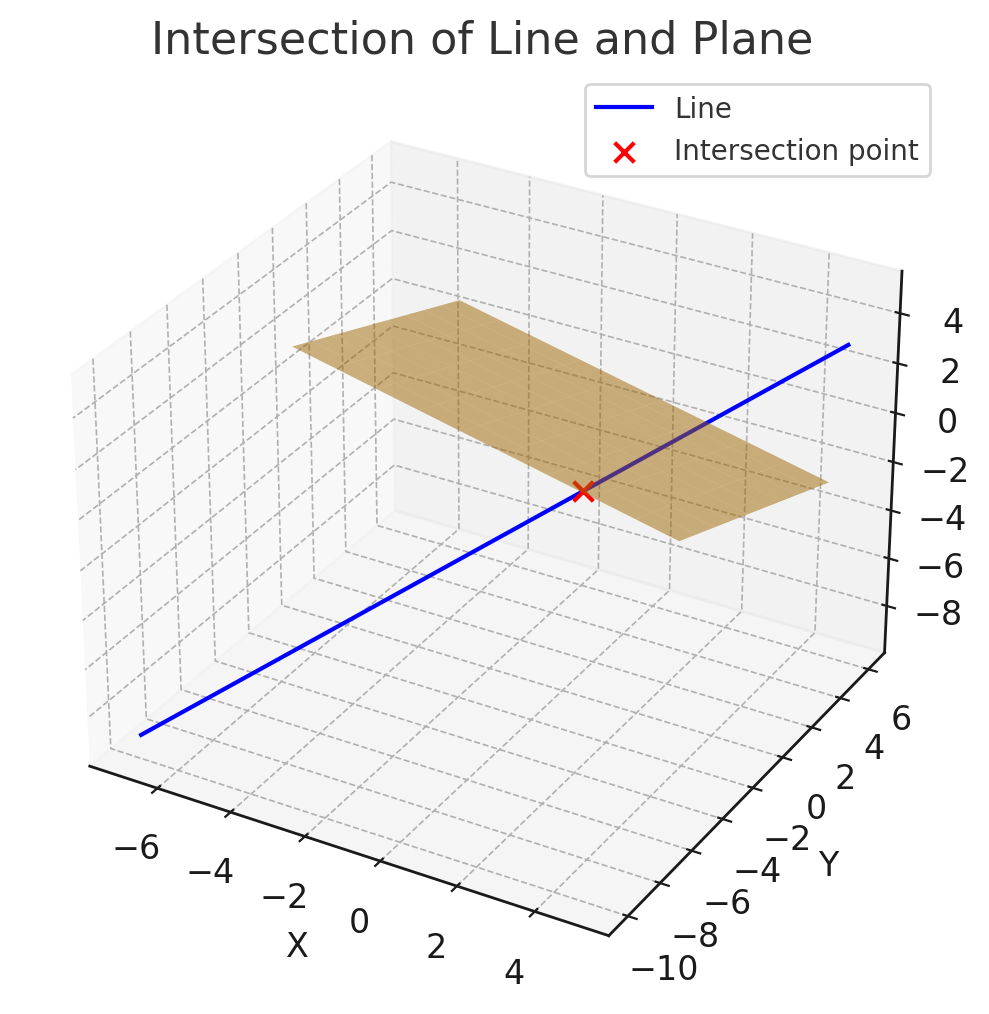
\includegraphics[width=\columnwidth, height=0.8\textheight, keepaspectratio]{beamer/figs/fig1.jpg}
   \label{fig:Beamer/figs/fig1.png}
\end{frame}

\end{document}
